Verkkotunnistautumiseen kehitettyjä protokollia hyödyntämällä käyttäjän tunnistetietoja (esim. käyttäjänimi ja salasana) ei tarvitse siirtää verkon yli ja web-palvelut voivat ulkoistaa tunnistautumisen erillisen palvelun tehtäväksi \cite{nisti}. Tällöin käyttäjä voi samalla identiteetillä tunnistautua useaan eri palveluun, ilman että hänen tarvitsee muistaa palvelukohtaisia tunnus- ja salasanayhdistelmiä \cite{open_identity}.

Tässä luvussa keskitytään keskitetyssä tunnistautumispalvelussa käytettyihin teknologioihin. Teknologiat ovat samoja, jotka ovat tällä hetkellä käytössä Internetin web-palveluissa \cite{facebook}. Ensimmäisessä alaluvussa käydään läpi yleisiä periaatteita koskien keskitettyä tunnistautumista. Toisessa alaluvussa tutustutaan tunnistautumisprotokolliin. Ensin käydään läpi protokollien yleisiä toimintaperiaatteita, minkä jälkeen esitellään tunnistautumisprotokollaksi soveltuvia standardeja. Tämän jälkeen tutkitaan SAML- ja OAuth-protokollien soveltuvuutta tunnistautumispalvelun toteuttamiseen.

Tunnistautumiseen liittyvien käsitteiden ymmärtäminen ennen protokollien yksityiskohtiin perehtymistä auttaa tunnistautumiseen liittyvien periaatteiden hahmottamista. Käsitteet ovat yleisluontoisia eivätkä kosketa vain tiettyjä protokollia. Protokollien yhteydessä käytetään käsitteitä asiakasohjelma (client), tunnistautumispalvelu (identity provider), suojattu resurssi (protected resource), valtuutustieto (credentials), valtuutusavain (authorization code) ja pääsyvaltuutus (access token) \cite{nisti}.

Asiakasohjelmalla tarkoitetaan web-palvelun käyttäjän pääteohjelmaa, jolla hän kirjautuu web-palveluun käyttäen keskitettyä tunnistautumispalvelua \cite{nisti}. Käytännössä asiakasohjelma on web-palvelun tapauksessa käyttäjän WWW-selain, joka pystyy tekemään uudelleenohjauksia sivustolta toiselle. Uudelleenohjaus on HTTP-pro\-to\-kol\-lan perustoiminnallisuutta, joten mikä tahansa HTTP/1.1-standardin WWW-selain käy asiakasohjelmaksi \cite{rfc2616}.

Tunnistautumispalvelu on web-palvelu, johon käyttäjä ohjataan tekemään tunnistautuminen. Onnistuneen tunnistautumisen jälkeen tunnistautumispalvelu ohjaa asi\-a\-kas\-oh\-jel\-man takaisin tunnistautumista pyytäneen palvelun määrittelemään osoitteeseen \cite{nisti}. Avoimen Internetin puolella tunnistautumispalvelu voi olla esimerkiksi Facebook tai LinkedIn.

Tunnistautumisprotokollien, kuten OAauth, yhteydessä suojatulla resurssilla tarkoitetaan resurssia, jonka käyttö vaatii tunnistautumisen ja käyttöoikeuden \cite{oauth2_0}. Yleisessä tapauksessa suojatulla resurssilla tarkoitetaan yksittäistä resurssia (esim. käyttäjän omistamaa valokuvaa), johon halutaan asettaa pääsyrajoituksia \cite{nisti}.

Valtuutustieto koostuu yksilöivästä tunnisteesta ja siihen liittyvästä salaisesta avaimesta. Tässä tutkielmassa valtuutustiedolla tarkoitetaan käyttäjän tunnusta ja salasanaa.

Kirjauduttuaan sisään tunnistautumispalvelimelle käyttäjä saa valtuutusavaimen, jonka hän lähettää eteenpäin suojatun resurssin omistajalle. Valtuutusavaimeen on kirjattu tieto käyttäjästä ja avaimen voimassaoloaika. Valtuutusavain ei pidä sisällään käyttäjän valtuutustietoja ja ainoastaan tunnistautumispalvelin osaa lukea sen \cite{nisti}. Saatuaan valtuutusavaimen käyttäjältä voi suojatun resurssin omistaja hakea pääsyvaltuuden.

Pääsyvaltuutus on tunnistautumispalvelimelta saatava yksilöivä tunniste, jonka avulla suojatun resurssin omistaja voi pyytää resurssia palvelimelta. Pääsyvaltuutus on voimassa tietyn ajan, jonka jälkeen se täytyy uusia tunnistautumispalvelimella \cite{nisti}. Pääsyvaltuutusta voidaan käyttää myös tunnistautumispalvelusta erillään olevien resurssien valtuuttamiseen. Esimerkiksi web-sovellus voi hakea tunnistautumispalvelulta pääsyvaltuuden, jolla se hakee valokuvia valokuvien jakopalvelusta \cite{facebook}.

Tunnistautumisessa on kolme osapuolta: asiakasohjelma, web-palvelu ja tunnistautumispalvelu \cite{nisti}. Osapuolet on esitetty kuvassa \ref{composition}, jossa on mukana myös tunnistautumispalvelun käyttämä käyttäjähallinta. Käyttäjähallinta voi olla myös osa tunnistautumispalvelua tai oma komponenttinsa. Tunnistautumisen kannalta sillä, onko käyttäjähallinta osa tunnistautumispalvelu vai erillinen komponentti, ei ole väliä.

\begin{figure}[ht]
\centering
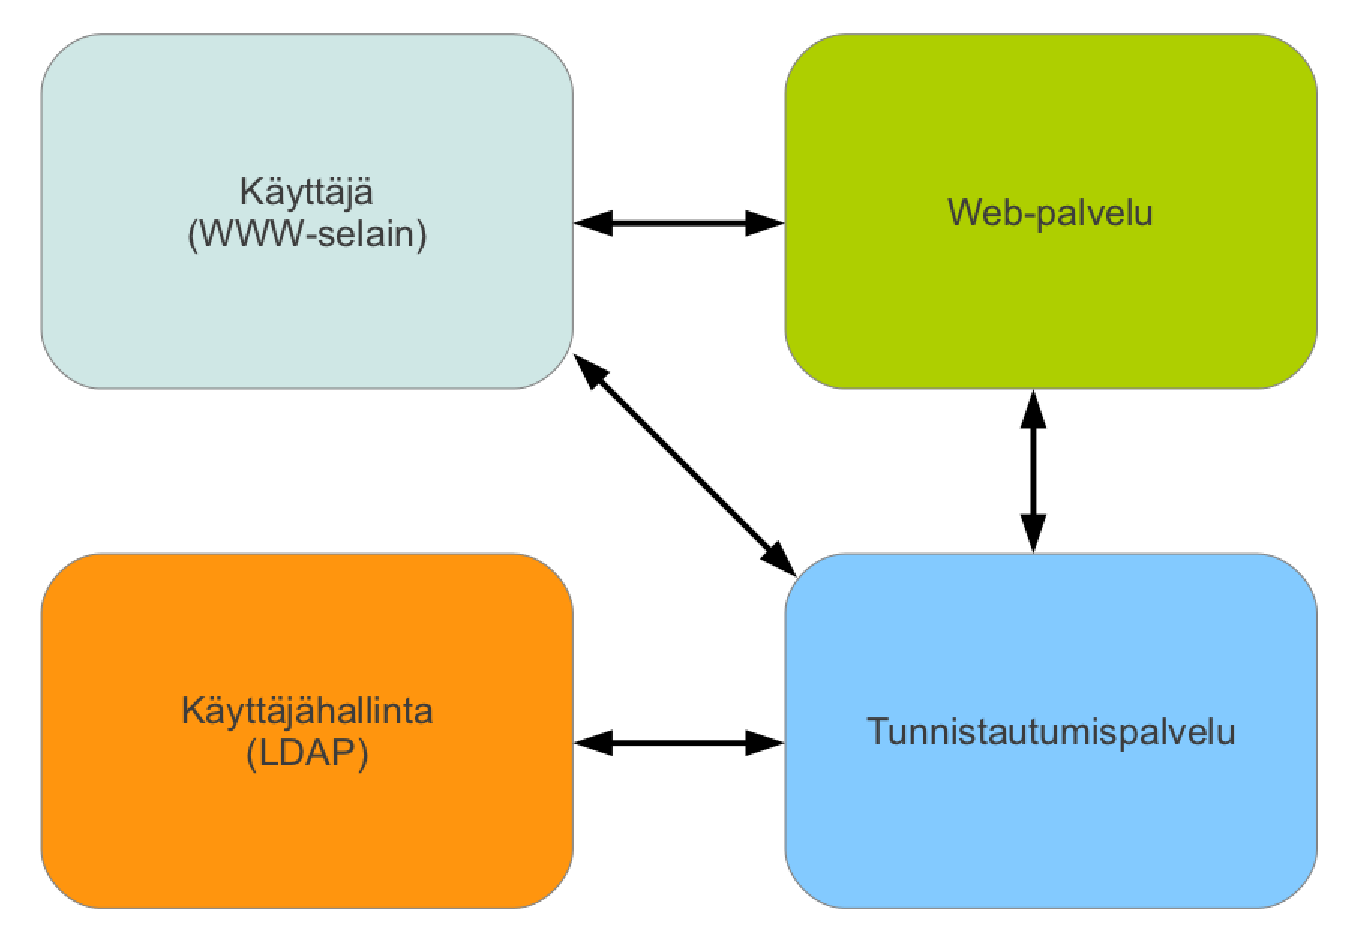
\includegraphics[width=0.7\textwidth]{teknologiat/composition.eps}
\caption{Keskitetyn tunnistautumisen osapuolet.}%
\label{composition}
\end{figure}

Ensimmäiseksi käyttäjä menee asiakasohjelmalla web-palveluun, joka pyytää tunnistautumista erillisessä tunnistautumispalvelussa. Käyttäjän asiakasohjelma ohjataan tunnistautumispalvelun sivulle, joka on yhteydessä organisaation käyttäjähallintaan. Käytetystä rajapintaprotokollasta riippuen käyttäjälle joko palautetaan todistus siitä, että hän on se jonka väittääkin olevansa tai avain, jonka avulla web-palvelu voi hakea käyttäjän tiedot tunnistautumispalvelulta.

Tunnistautumisprotokollia (kuten SAML, OpenID) käytettäessä käyttäjälle palautetaan valtuutustieto, joka on tunnistautumispalvelun allekirjoittama. Tämä valtuutustieto vahvistaa käyttäjän identiteetiksi sen, joka hän väittää olevansa \cite{nisti}.

Pääsynhallintaprotokollien (esim. OAuth) kohdalla käytetään ns. näennäistunnistautumista (pseudo authentication) \cite{distributed_web_security}. Tällöin web-palvelu voi hakea valtuutusavaimella käyttäjän tiedot tunnistautumispalvelusta. Käyttäjän identiteettiä ei siis suoraan varmenneta väitetyksi, mutta koska käyttäjällä on hallussaan avain, jolla pääsee hänen tietoihin käsiksi, oletetaan käyttäjän olevan se, jonka tiedot avaimella saadaan.

Useimmat tunnistautumisen vaiheet tapahtuvat käyttäjältä näkymättömissä selaimen uudelleenohjauksella. Käyttäjälle näkyvä vaihe on kirjautuminen tunnistautumispalvelulle, jolloin käyttäjältä pyydetään käyttäjätunnus ja salasana. Käyttäjän syötettä vaativat vaiheet on esitetty aiemmassa kuvassa \ref{facebook_login}.